\chapter{Ionization}
\label{chap:ionization}

In this chapter the model presented before is modified by introducing a small oscillating  external voltage. This perturbation allows the Majorana state to excite into continuum --- the process we will call ionization. The main goal here is to find the ionization rate when the typical size of the photon is much smaller than the spectrum gap.  Only regime with $ \abs{g_L}\ll g_R $ is considered --- this significantly simplifies the calculation, but still exhibits non-trivial physics with a number of different subregimes. 

\section{Introducing the perturbation}

 The perturbation is introduced as an oscillating	 voltage applied to the junction. This alters the Hamiltonian (\ref{full_hamiltonian}) in two ways --- by the modification of the chemical potentials $ \mu_L, \mu_R $ and by making the superconducting phase difference $ \varphi=\phi_R-\phi_L $ time dependent. The second effect is governed by the Josephson relation:
\begin{gather}
	U\br{\tau}
	=
	\frac{\hbar}{2e}
	\frac{\partial\varphi\br{\tau}}{\partial \tau}
\end{gather}

The ionization voltage is assumed to be small compared to other energy parameters, and this smallness is present in both effects. However, if the frequency $ \omega $ of voltage is also small, the perturbation in $ \Delta $ induced by the second effect will have additional big multiplier $ \frac{\Delta}{\omega} $ and will dominate the perturbation in $ \mu $. In this chapter only this regime is considered.

Time dependence of phase difference is introduced as:
\begin{gather}
	\varphi\br{\tau}=\varphi_0+\alpha\cos\omega \tau
\end{gather}
where $ \varphi_0 $ is an initial time independent phase difference and $ \alpha\ll1 $ is the amplitude of phase oscillations.

As was shown in section  \ref{sec:elimintaing_long-wave}, there is a gauge transform $ U_\phi $, which  redistributes the phase difference between the wires, so the phase in a given wire can have any value. This ambiguity just reflects a  fact, that only phase difference $ \varphi $ is an observable quantity, but not the phases $ \phi_L $, $ \phi_R $ separately. However, when treating the time dependent  phase difference this gauge transform also becomes time-dependent. After its application the additional term $ \dot{U}_{\phi\br{\tau}}U_{\phi\br{\tau}}^\dagger \propto \dot{\phi}\br{\tau}$ will appear, but, as $ \omega $ is small, it can be neglected. The corresponding condition on $ \omega $ will be established in section \textbf{ENTER SECTION}  

As the term $ \dot{U}_{\phi\br{\tau}}U_{\phi\br{\tau}}^\dagger \propto \dot{\phi}\br{\tau}$ is negligible, we again can gauge all the phase difference into the boundary condition. Now the boundary condition is time-dependent. It's not very convenient, and to avoid dealing with it we reformulate the problem in terms  of tunnel Hamiltonian, which allow us to treat both tunneling and time dependence simultaneously via perturbation theory.


\if 0

We introduce the time-dependent phases as: $ \phi_L=-\frac{\varphi_0}{2}-\frac{\alpha}{2}\cos \omega t $, $ \phi_R=-\phi_L=\frac{\varphi_0}{2}+\frac{\alpha}{2}\cos \omega t $. Thus the superconducting terms in the wire Hamiltonians alter: $ \Delta_{\pm\frac{\varphi}{2}} \to\Delta_{\pm\frac{\varphi}{2}\pm \frac{\alpha}{2}\cos \omega t} $. Decomposing them in small $ \alpha $ one can explicitly write the perturbation and try to compute the ionization rate. However this way appears to be quite difficult as the overlaps of all the states 
present in both wires and at first it seems that the Majorana states has too much ways to ionize. To avoid this difficulty, the tunnel Hamiltonian approach is used.

\fi

\section{Tunnel Hamiltonian approach}
\label{sec:tunnel_hamiltonian}
The main idea of this method is to hide all the time dependence and the tunnel effect in one single operator. To do so we need to rewrite the Hamiltonian as $ H=H_L+H_R+H_T $, where $ H_{L,R} $ are the Hamiltonians of the left and right wire without any contact (corresponding to zero tunneling: $ t=0 $), and $H_T  $ is a tunnel Hamiltonian both containing the time dependence and mixing the wavefunctions from different wires. 
Here the following notation is used: the Hamiltonians $ H_L $, $ H_R $ and $ H_T $ are 8x8 matrices in combined Nambu-Gorkov and LR-space. In LR-space they have the following form:
\begin{gather}
\label{tunnel_Hamiltonian_formalizm}
	H_L
	=
	\begin{pmatrix}
	h_L & 0 \\
	0 & 0
	\end{pmatrix}_{LR}
	\quad
	H_R
=
\begin{pmatrix}
0 & 0 \\
0 & h_R
\end{pmatrix}_{LR}
\quad
	H_T
=
\begin{pmatrix}
0 & h_{LR} \\
h_{RL} & 0
\end{pmatrix}_{LR}	
\end{gather}
The Hamiltonians $ h_L $ and $ h_R $ eventually coinside with (\ref{bulk_Hamiltonian}) with zero boundary condition. The Hamiltonian $ h_{LR}=h_{Rl}^\dagger $ in unknown --- the goal is to make it in a way the corrections for the wavefunctions are restored . This wavefunctions and their  first tunneling corrections are listed in  appendix \ref{app:wavefunctions_with_corrections}.

The derivation of tunnel Hamiltonian matrix elements is presented in appendix \ref{app:tunnel}. Using the notation  $ \big|\gamma_{0}\,\big> $ for Majorana state and $ \big|\varepsilon,L_{0}\,\big> $, $ \big|\varepsilon,R_{0}\,\big> $ for continuous spectra, we have the following:
\begin{gather}
H_T=
\left(e^{i\frac{\varphi}{2}}+e^{-i\frac{\varphi}{2}}\right)
\tilde{H}_{T}
=
\left(e^{i\frac{\varphi}{2}}+e^{-i\frac{\varphi}{2}}\right)
\begin{pmatrix}
0 & \tilde{h}_{LR} \\
\tilde{h}_{RL} & 0
\end{pmatrix}
\\
\label{tunnel_matrix_elements_maj-cont}
	\big<\gamma_{0}\,\big|\tilde{h}_{RL}\big|E,L_{0}\,\big>
	=
	4\sqrt{ug_{R}}
	t\zeta^{2}
	f\br{\frac{E}{\abs{g_L}}}
	\\
	\label{tunnel_matrix_elements_cont-cont}
	\big<\epsilon,R_{0}\,\big|\tilde{h}_{RL}\big|E,L_{0}\,\big>
	=
	-16u\zeta^{2}t
	f\br{\frac{E}{\abs{g_L}}}
	f\br{\frac{\varepsilon}{g_R}}
\end{gather}
where $ f\br{x}=\sqrt{x^2-1}\br{x+\sqrt{x^2-1}} $. 

 The fact, that all energy dependences here are described by a single function $ f\br{x} $ insinuates that maybe it's possible to make this calculations in a more beautiful way.

\section{Ionization rate for $ g_R\gg\abs{g_L} $}


\subsection{Time dependence of perturbation}

To obtain the ionization rate one should treat $ H_T $ as perturbation. For unperturbed system, described with $ H_0=H_R+H_L $, the electrons cannot get from wire to another, but $ H_T $ allows these processes, so the ionization can be described as a set of jumps from right to left wire (see fig. \ref{fig:tunneling}).

\begin{figure}[H]
	\centering
	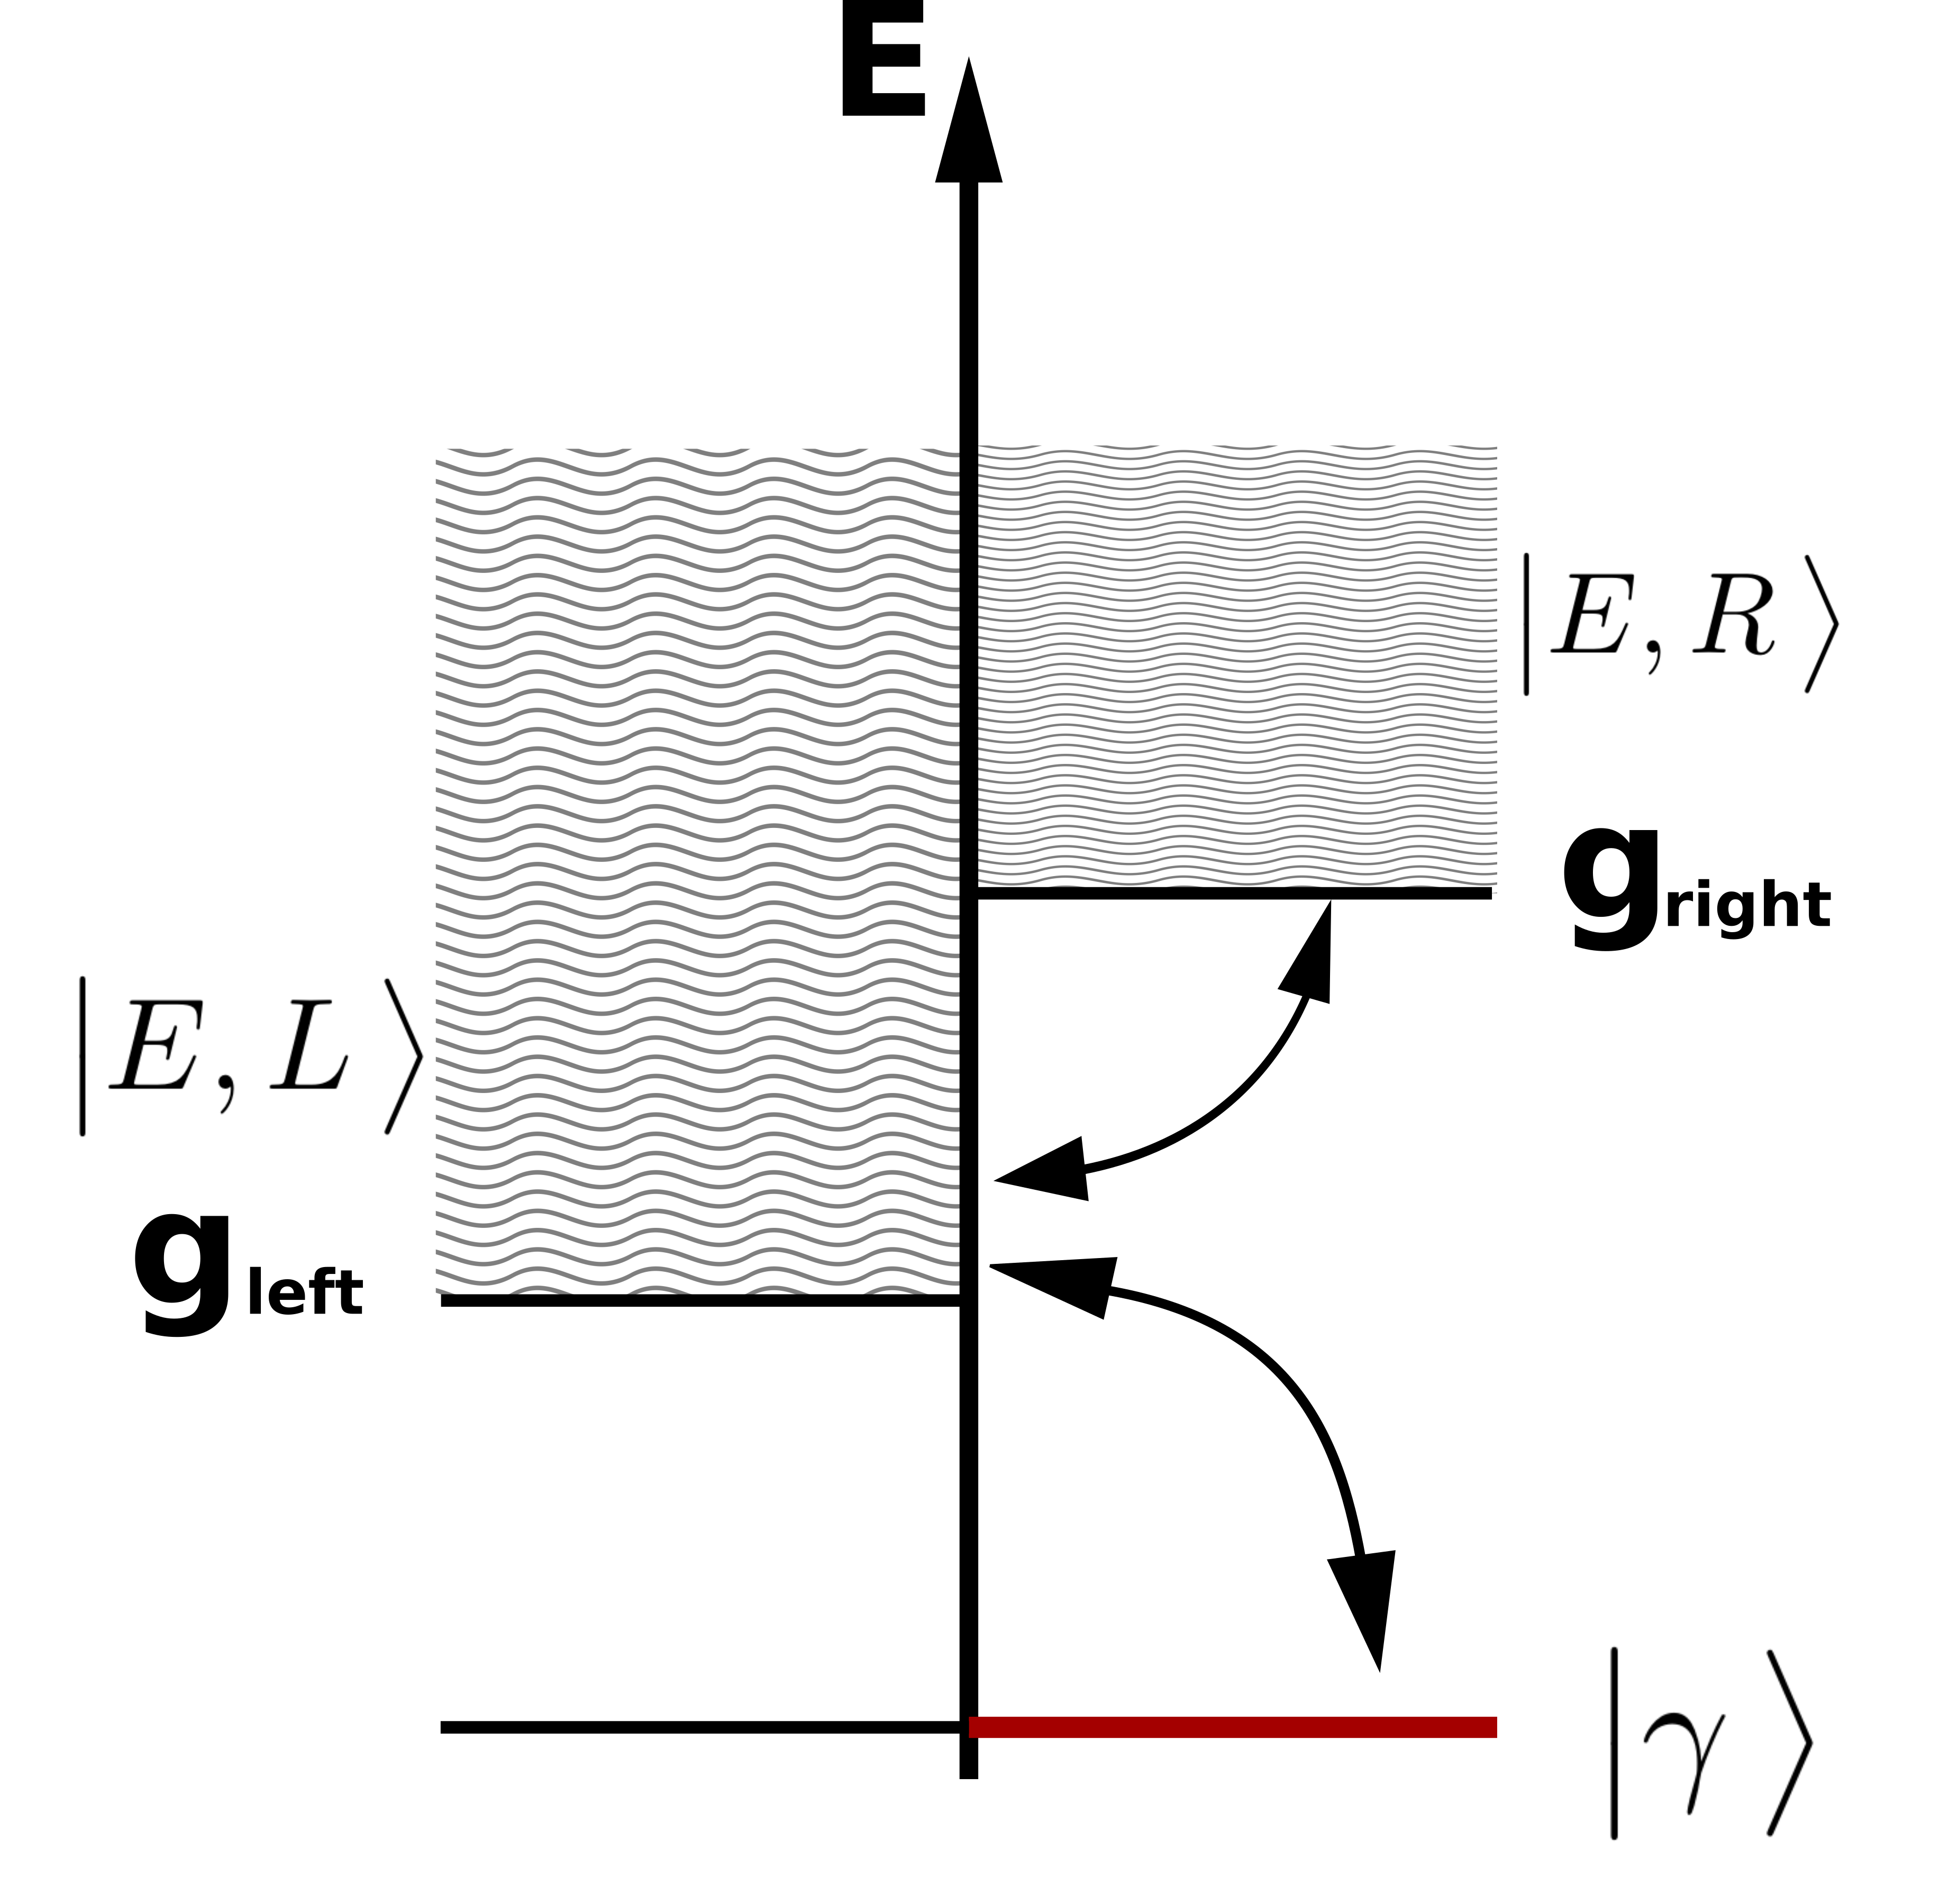
\includegraphics[width=0.65\linewidth]{images/tunneling}
	\caption{Ionization processes in terms of tunnel Hamiltonian}
	\label{fig:tunneling}
\end{figure}

The approach to multiphoton ionization is described in Appendix \ref{app:multiphoton ionization}.  The first step is to decompose the  perturbation in Fourier series in frequencies. From  (\ref{tunnel_matrix_elements_maj-cont}) one finds, that $ H_T\propto\cos\frac{\varphi\br{\tau}}{2} $ with $ \varphi\br{\tau}=\varphi_{0}+\alpha\cos\omega \tau $. Using $ \alpha\ll1 $, we write:
\begin{multline}
	e^{\frac{i\varphi\br{\tau}}{2}}+e^{-\frac{i\varphi\br{\tau}}{2}}\simeq e^{i\frac{\varphi_{0}}{2}}\sum_{n}\frac{(i\alpha)^{n}}{2^{n}n!}(e^{in\omega \tau}+e^{-in\omega \tau})+c.c=
	\\
	=\sum_{n}\frac{\alpha{}^{n}}{2^{2n-1}n!}(e^{in\omega \tau}+e^{-in\omega \tau})\cos\left(\frac{\varphi_{0}}{2}+n\frac{\pi}{2}\right)
\end{multline}
so:
\begin{gather}
	H_{T}=
	\sum_n
	H_{T,n}
	\br{
	e^{in\omega\tau }
	+
	e^{-in\omega\tau }
	},
	\qquad
	H_{T,n}
	\approx
	\sum_{n}	
	\frac
	{\alpha^{n}}
	{2^{2n-1}n!}
	\cos\left(\frac{\varphi_{0}}{2}+n\frac{\pi}{2}\right)
	\tilde{H}_{T}
\end{gather}
The same decomposition is valid for $ LR $ matrix elements of $ H_T $:
\begin{gather}
h_{LR}=
\sum_n
h_{LR,n}
\br{
	e^{in\omega\tau }
	+
	e^{-in\omega\tau }
},
\qquad
h_{LR,n}
\approx
\sum_{n}	
\frac
{\alpha^{n}}
{2^{2n-1}n!}
\cos\left(\frac{\varphi_{0}}{2}+n\frac{\pi}{2}\right)
\tilde{h}_{LR}
\end{gather}
Then the rate is given by (see Appendix \ref{app:multiphoton ionization}):
\begin{gather}
\label{ionization_key}
\mathcal{I}
\sim
\frac{|\langle\mathcal{E}|w_{\mathcal{E}}|\gamma\rangle|^{2}}{N(\mathcal{E})},
\qquad
w_{\mathcal{E}}(E)
=
\sum_{\{n_{i}\}:\mathcal{E}}H_{T,n_{N}}\prod_{j=1}^{N-1}G_{0}\left(E+\sum_{s=1}^{j}\omega_{n_{s}}\right)H_{T,n_{j}}
\end{gather}
here sum is taken over all sets $ \{n_i\}:\mathcal{E} $ so that $ \sum_{i} \omega_{n_i}=\mathcal{E}=\min[g_R, \abs{g_L}]$. Each term in sum (\ref{ionization_key}) corresponds to some way (i.e. trajectory) to absorb photons with energies $ \omega_{n_i} $, such that the total absorbed energy is equal to spectrum gap.

For unperturbed Green function we take a notaion:
\begin{gather}
	G_0\br{E}
	=
	\begin{pmatrix}
	G_L\br{E} & 0 \\
	0 & G_R\br{E}
	\end{pmatrix}_{LR}.
\end{gather}

In this section the focus is on the case where the topological gap is much larger than the trivial one: $ \abs{g_L}\ll g_R $. Then the right continuum has high energies and does not participate in the ionization process. Indeed,
\begin{gather}
	h_{LR} G_R\br{\epsilon} h_{RL}
	=
	\frac{h_{LR}|\gamma\rangle\langle\gamma|h_{RL}}{\epsilon}
	+
	\intop_{|E|>g_{R}}
	\frac{h_{LR}|E,R_0\rangle\langle E,R_0|h_{RL}}{\epsilon-E}\frac{dE}{N_{R}(E)}
\end{gather}
So, when $ g_{R}\gg\epsilon\sim \abs{g_L} $, the second term is small and can be neglected. Then, the product $ \dots h_{RL}G_L\br{E}h_{LR}G_R\br{E}h_{RL}\dots $ factorizes into individual factors, which we denote as $ J_{nm}\br{E}\equiv\langle\gamma|h_{RL,n}G_L\br{E}h_{LR,m}|\gamma\rangle $.

\subsection{Factorizing $ w_\mathcal{E} $}
\label{sect:factorizeing_w}

As each entry in the sum within $ w_{\mathcal{E}} $ has the form $ \dots h_{lR}G_R\br{E}h_{RL}G_L\br{E}h_{LR}\dots $, we have:
\begin{gather}
	\sqrt{\mathcal{I}}\propto
	\sum_N \sum_{\{n_i\}_M^N}
	J_{n_1 n_{2}}
	J_{n_3 n_{4}}
	\cdots
	J_{n_{N-1}n_{N}}
\end{gather}
Here $ N $ has the meaning of total number of absorbed photons, $ M $ is the integer closest to $ \frac{\abs{g_L}}{\omega }$ , and the second sum is taken over all sets $ \{n_i\}_M^N $ of $ N $ items such that $ \sum_{i=1}^N n_{i} = M$. We set, the number $ N $ to be even, hiding the last photon into unimportant prefactor.

 The $ n $,$ m $-dependence factors out:
\begin{gather}
J_{nm}\br{E}
=
	\frac{\alpha^{n+m}}
	{2^{2\br{n+m}-2}n!m!}
	\cos\left(\frac{\varphi_{0}}{2}+n\frac{\pi}{2}\right)
	\cos\left(\frac{\varphi_{0}}{2}+m\frac{\pi}{2}\right)
	Q_0\br{E}
\end{gather}
\begin{gather}
	Q_{0}(E)
	=
	\langle\gamma|\tilde{h}_{RL}G_L(E)\tilde{h}_{LR}|\gamma\rangle
	\equiv
	\intop_{cont.}\frac{|\langle\gamma|\tilde{h}_{LR}|\epsilon\rangle|^{2}}{E-\epsilon}\frac{d\epsilon}{N_L(\epsilon)}
\end{gather}

On each ionization step  the particle can move to the state with energy $ E $ or $ -E $, so:
\begin{gather}
	Q_{0}(E)
	=
	2E\intop_{|g_{L}|}^{\infty}\frac{|\langle\gamma|\tilde{h}_{RL}|\epsilon\rangle|^{2}}{E^{2}-\epsilon^{2}}\frac{d\epsilon}{N_L(\epsilon)}
\end{gather}
recalling (\ref{tunnel_matrix_elements_maj-cont}), we obtain:
\begin{gather}
\label{ionization_brick}
		Q_{0}(E)
		=
		ET\frac{\left[-1+\sqrt{1-\lambda^{2}}\right]}{\lambda^{2}}
\end{gather}
where $ \lambda = \frac{E}{\abs{g_L}} $, $ T=\frac{g_R\br{\zeta^2t}^2}{\abs{g_L}} $. We consider $ T\ll 1$, so the systems remains in a strong tunneling limit.

Thus, the elementary block  in our product for small enough $ n $ becomes:
\begin{gather}
	\frac{J_{nm}}{E+n\omega}
	\approx
	\frac{J_{nm}}{E}
	=
	\br{\frac{\alpha}{4}}^{n+m}
	B_n B_m T
	\frac{-1+\sqrt{1-\lambda^2}}{\lambda^2}
\end{gather}
where
\begin{gather}
	B_n=
	\frac{2}{n!}\cos\br{\frac{\phi_0}{2}+\frac{\pi n}{2}}
\end{gather}

The prefactor $  \br{\alpha/4}^{n+m} $ yields $ (\alpha/4)^{\mathcal{E}/\omega} $ for any trajectory and therefore do not affect summation and optimization. Thus one has $ B_{n}B_{m}T\frac{-1+\sqrt{1-\lambda^{2}}}{\lambda^{2}} $ to optimize.

Now consider a slice of the ionization process, i.e. a part of the full ionization product, which runs from energy $ E $ to $ E+\Delta E $ where $ \Delta E=M\omega $ with a large M. One can assume that within that process, a large number N of photons is absorbed, but energy does not change significantly, $ \Delta E\ll E $, so that $ \lambda $ can be considered a constant within that process. 

This approach is invalid, if the optimal photon energy is larger  than the slice size. If this happens, one needs to enlarge the slice until it reaches the energy of optimal photon. It cannot be done, when the optimal photon energy is equal or larger than spectrum gap. This case will be treated separately in section (\textbf{ENTER SECTION}).

For now, denoting
\begin{gather}
\label{T_lambda_def}
	T_{\lambda}=-4T\frac{\left[-1+\sqrt{1-\lambda^{2}}\right]}{\lambda^{2}}
\end{gather}
we rewrite:
\begin{gather}
\label{ionization_super_formula_sum}
\mathcal{J}\br{\lambda}
\equiv
\sum_N
\sum_{\{n\}_{N}^{M}}\frac{	J_{n_1 n_{2}}
	J_{n_3 n_{4}}
	\cdots
	J_{n_{N-1}n_{N}}}{E^{\frac{N}{2}}}
=
\left(\frac{\alpha}{4}\right)^{M}
\sum_N
\br{-T_{\lambda}}^{\frac{N}{2}}
\mathcal{J}_N
\\
\label{ionization_super_formula}
\mathcal{J}_N
=
\sum_{\{n\}_{N}^{M}}\prod_{i=1}^{N}\frac{\cos(\frac{\varphi_{0}}{2}+\frac{\pi n_{2i}}{2})}{n_{i}!}
\end{gather}

So to obtain the ionization rate up to a prexponential constant, one should compute $ \mathcal{J}\br{\lambda} $ and take the product 
$ \underset{\lambda_k}{\prod} \mathcal{J}\br{\lambda_k}$ where $ \lambda_k $ corresponds for the $ k $-th slice of the ionization process.  
\subsection{Estimation for optimal photon number}
We begin dealing with (\ref{ionization_super_formula_sum}) by finding the optimal photon number $ N_* $. This number corresponds to the largest term in the sum (\ref{ionization_super_formula_sum}).

The first step is to use Poisson summation formula:
\begin{gather}
	\sum_{n=-\infty}^\infty
	\delta\br{x - n}
	=
	\sum_{k=-\infty}^\infty
	e^{2i\pi x}
\end{gather} 
so:
\begin{multline}
	\mathcal{J}_N
	=
	\\
	=
	\br{
	\sum_{k_1=-\infty}^\infty
	\cdots
	\sum_{k_{N-1}=-\infty}^\infty
	}
	\prod_{i=1}^{N-1}
	\br{
	\int d x_i
	e^{2i \pi k_i x_i}
	\frac
		{	
			\cos
			\br{
				\frac{\varphi_0}{2}
				+
			\frac{\pi x_i}{2}
			}
		}
		{\Gamma\br{x_i+1}}
	}
	\frac
{
	\cos
	\br{
		\frac{\varphi_0}{2}
		+
		\frac{\pi x_{N}}{2}
	}
}
{\Gamma\br{x_{N}+1}}
\end{multline}
where $ x_{N} \equiv M - \sum_{i=1}^{N-1} x_i$. This can be rewritten as:
\begin{gather}
		\mathcal{J}_N
		=
		\frac{1}{2^{N}}
		\sum_{\mathbf{k}}
		\br{
			\sum_{s_1=\pm 1}
			\cdots
			\sum_{s_{N}=\pm1}
		}
	\br{
		\prod_{i=1}^{N-1}
		\int
		d x_i
	}
	e^{S[\mathbf{x}]}
\end{gather}
with 
\begin{gather}
\label{ionization_saddle_action}
	S[\mathbf{x}]
	=
	-
	\sum_{i=1}^{N}
	\log \Gamma\br{x_i+1}
	+
	2i\pi\sum_{i=1}^{N-1}
	k_i x_i
	+
	i
	\sum_{i=1}^{N}
	s_i
	\br{\frac{\varphi_0}{2}
	+
	\frac{\pi x_i}{2}	
	}
\end{gather}
As $ N $ and $ M $ are large, we assume that $ x_i $ at saddle points are also large, so the Stirling approximation is relevant: $\log \Gamma\br{x} \approx x\log x - x $. As we just make the estimation for saddle point position, we can neglect all the terms in (\ref{ionization_saddle_action}) except for the first one and get (recall, that $ x_{N}
= M-\sum_{i=1}^{N-1}x_i $):
\begin{gather}
	\frac{\partial}{\partial x_i}
	S[\mathbf{x}]
	\approx
	\log{x_{N}}-\log{x_i}
\end{gather}
So, at the saddle point all $ x_i $ are equal to $ \frac{M}{N} $. 

Each $ x_i $ corresponds to  it's own $ n_i $. In saddle point approximation we can take only terms with $ n_i = x_i^{\mathrm{saddle}} $ in sum (\ref{ionization_super_formula}). Than the sum (\ref{ionization_super_formula_sum})  becomes:
\begin{gather}
\label{ionization_sum_saddle}
	\mathcal{J}\br{\lambda}
	\approx
	\sum_N
	A_N
	\br{-T_\lambda}^\frac{N}{2}
	e^{-
		M
		\log\frac{M}{N}
	}
=
\sum_N
A_N
\br{-1}^\frac{N}{2}
e^{\frac{N}{2}
\log T_\lambda
-
M\log\frac{M}{N}
 }
\end{gather}
with relatively slow function $ A_N $. 

It's easy to see, that the biggest term in (\ref{ionization_saddle_action}) corresponds to the $ N_*=2M/\log\frac{1}{T_\lambda} $. This is the optimal photon number  for the slice  from $ E $ to $ E+\Delta E $ of energy range with $ E=\abs{g_L}\lambda  $ and $ \Delta E = \omega M $. Consequentially the optimal photon size is given by $ n_*=\frac{M}{N_*}=\frac{1}{2}\log\frac{1}{T_\lambda} $. From (\ref{T_lambda_def}) we see, that $ T_\lambda $ differs from $ T $ by a smooth depending on $ \lambda $ prefactor phonot. We introdice a global optimal photon size $ n_T\equiv\log\frac{1}{T} \gg1$ and find, that $ n_* \sim n_T $. It's important to note, that $ n_* $ doesn't depend on the energy slice size $ M $, being an intensive parameter of the process.

\subsection{Two regimes of factorized ionization}
To treat (\ref{ionization_super_formula}) more accurately it's convenient to use the multinomial formula:
\begin{gather}
	\frac{d^M}{dx^M}
	\prod_{i=1}^N f_i\br{x}
	=
	\sum_{\{n_i\}_{N}^{M}}
	\begin{pmatrix}
	M
	\\
	n_1,n_2,\dots,n_N
	\end{pmatrix}
	\prod_{i=1}^N
	\frac{d^{n_i}}{dx^{n_i}}
	f_i
\end{gather}
For the cosine product it can be applied in a following way:
\begin{gather}
	\sum_{\{n\}_{N}^{M}}\prod_{i=1}^{N}\frac{\cos(\chi+\frac{\pi n_{i}}{2})}{n_{i}!}=\sum_{\{n\}_{N}^{M}}\prod_{i=1}^{N}\frac{D_{\chi}^{n_{i}}}{n_{i}!}\cos\chi=\frac{1}{M!}D_{\chi}^{M}\cos^{N}\chi
\end{gather}
where $ \chi=\frac{\varphi_0 }{2}$. Then some algebra should be used:
\begin{multline}
\label{after_multinomial}
	\frac{1}{M!}D_{\chi}^{M}\cos^{N}\chi=
	\frac{1}{2^{N}M!}D_{\chi}^{M}\sum_{k=0}^{N}C_{k}^{N}e^{i\chi(N-2k)}
	=
	\frac{e^{i\chi N+iM\pi/2}}{2^{N}M!}\sum_{k=0}^{N}C_{k}^{N}(N-2k)^{M}e^{-2ki\chi}
\end{multline}
So:
\begin{gather}
\label{sum_after_multinomial}
	\mathcal{J}_N
	=
		\frac{e^{i\frac{\varphi_0}{2} N+iM\pi/2}}{2^{N}M!}\sum_{k=0}^{N}C_{k}^{N}(N-2k)^{M}e^{-ik\varphi_0}
\end{gather}

Now, in the sum, the ratio of consecutive summands is $ \frac{a_{k+1}}{a_{k}}=\frac{C_{k+1}^{N}}{C_{k}^{N}}\left(\frac{N-2k-2}{N-2k}\right)^{M} $. This ratio can be larger or less than unity.
When $ \frac{a_{k+1}}{a_{k}} <1 $ for any $ k<\frac{N}{2} $, the largest ratio is  $ \frac{a_{1}}{a_{0}}=N(\frac{N-2}{N})^{M}\simeq Ne^{-2M/N} $, so only $ a_0 $ and $ a_N $ should be taken into account. 
The summand $ a_0  \propto e^{\frac{iN\varphi_0}{2}}$ corresponds to tunneling $ N/2 $ electrons to the left and  $ N/2 $ holes to the right, while the $ a_N\propto e^{\frac{-iN\varphi_0}{2}} $ corresponds to tunneling $ N/2 $ electrons to the right and  $ N/2 $ holes to the left. So, the regime with only these two terms being present is a pure Andreev reflection regime. Taking $ N=N_* $, we rewrite the condition $ \abs{\frac{a1}{a_0}}\ll 1 $ as $ M\ll n_T e^{n_T} \sim T \log\frac{1}{T} $. 

When this condition is broken, the largest terms in (\ref{sum_after_multinomial}) are not $ a_0 $ and $ a_N $. This corresponds to some mixture of Andreev and normal reflections and should be treated separately.


\subsection{Pure Andreev reflection regime}
\label{sect:pure_MAR}

In pure Andreev the sum (\ref{sum_after_multinomial}) can be rewritten as:
\begin{gather}
\label{pure_MAR_sum}
	\mathcal{J}\br{\lambda}
	\approx
	\left(\frac{\alpha}{4}\right)^{M}\sum_{N}(-T_{\lambda})^{N/2}\frac{N^{M}}{2^{N-1}M!}\cos\left(\frac{N\varphi_0}{2}+\frac{M\pi}{2}\right)
\end{gather}
The preexponent is not the object of interest, while the fixed parity of $ N $ should be taken into account. Here we set $ N=2K $. With the help of polylogarithmic function
\begin{gather}
	\li_s\br{z}
	=
	\sum\frac{z^k}{k^s}
\end{gather}
we rewrite (\ref{pure_MAR_sum}) as:
\begin{multline}
\label{pure_MAR_to_polylog}
	\mathcal{J}\br{\lambda}=
	\left(\frac{\alpha}{4}\right)^{M}\sum_{K=1}^{\infty}(-T_{\lambda})^{K}\frac{(2K)^{M}}{2^{2K-1}M!}\cos\left(\varphi_{0}K+\frac{M\pi}{2}\right)=
	\\
	=\frac{2}{M!}\left(\frac{\alpha}{4}\right)^{M}\Re\left[i^{M}\sum_{K}(-T_{\lambda})^{K}\frac{(2K)^{M}}{2^{2K}}e^{i\varphi_{0}K}\right]=\\=\frac{2^{M+1}}{M!}\left(\frac{\alpha}{4}\right)^{M}\Re\left[i^{M}\li_{-M}\left(\frac{T_{\lambda}}{4}e^{i(\varphi_{0}+\pi)}\right)\right]
\end{multline}

The polylogarithmic function can be rewritten in the following useful way
\begin{gather}
\label{polylog_useful_formula}
	\li_{s}(e^{\mu})=\Gamma(1-s)\sum_{r\in\mathbb{Z}}(2r\pi i-\mu)^{s-1}
\end{gather}

Substituting, we get
\[
\li_{-M}\left(\frac{T_{\lambda}}{4}e^{i(\phi_{0}+\pi)}\right)=\Gamma(1+M)\sum_{r\in\mathbb{Z}}\left(i[2r\pi-\pi-\varphi_{0}]+\log\frac{4}{T_{\lambda}}\right)^{-M-1}
\]

Denoting $\log\frac{4}{T_{\lambda}}=n_{\lambda}$ we have the ratio
of consecutive terms in the sum (assuming they are not too far from
the largest term):
\[
\left|\frac{a_{r+1}}{a_{r}}\right|\sim\left(\frac{n_{\lambda}^{2}+(\gamma_{r}+2\pi)^{2}}{n_{\lambda}^{2}+\gamma_{r}^{2}}\right)^{-1-M}\sim\left(1+\frac{2\pi(2\pi+2\gamma_{r})}{n_{\lambda}^{2}+\gamma_{r}^{2}}\right)^{-M}\sim\exp\left[\frac{4\pi M(\pi+\gamma_{r})}{n_{\lambda}^{2}}\right]
\]

where $\gamma_{r}=i(2r\pi-\pi-\varphi_{0})$. There are two values of
$r$ for which $|\pi+\gamma_{r}|$ is smallest, for the rest it is
not smaller than $2\pi$ so that the rest of the terms are smaller
by at least 
\[
\exp\left[-\frac{8\pi^{2}M}{n_{\lambda}^{2}}\right]
\]

This leads us to three additional subcases. When $ M \gg n_\lambda^2\sim n_T$, the sum over $ r $ is dominated by the  largest terms: they correspond to $ r=0,1 $ for $ -\pi<\varphi_0<\pi $. The small number of terms in (\ref{polylog_useful_formula}) corresponds to the large number of terms in (\ref{pure_MAR_to_polylog}), so in this case not only the trajectories with $ N_* $ contributes to ionization, but also the large number of neighboring ones.

When $ M\ll n_\lambda^2 $, the formula (\ref{polylog_useful_formula}) isn't useful. Instead we look directly at (\ref{pure_MAR_to_polylog}) and find, that if $ M<n_T $ only first term is relevant --- which is one photon case, treated in section \textbf{ENTER SECTION}. When $ n_T\ll M\ll n_T^2 $, the maximum term in (\ref{pure_MAR_to_polylog}) is at $ N_*\sim\frac{M}{n_T} $.

The subcases $ n_T \ll M\ll n_T^2 $ and $ n_T^2 \ll M\ll n_T e^{n_T} $ are presented below.

\subsubsection{ Subcase $ n_T^2 \ll M\ll n_T e^{2n_T} $}

In this case  we have

\begin{gather}
	\li_{-M}\left(\frac{T_{\lambda}}{4}e^{i(\varphi_{0}+\pi)}\right)\simeq M!\left(\frac{1}{(n_{\lambda}+i(\pi-\varphi_{0}))^{M+1}}+\frac{1}{(n_{\lambda}+i(-\pi-\varphi_{0}))^{M+1}}\right)
\end{gather}

For $ \varphi_0<0 $ only the first term should be left, while for the $ \varphi_0>0 $ only the the second one. Thus the answer, obviously, depends on $ \varphi_0 $ and can be obtained only for the case, say $ \varphi_0>0 $.

So we set:

\begin{gather}
\li_{-M}\left(\frac{T_{\lambda}}{4}e^{i(\varphi_{0}+\pi)}\right)
\simeq \frac{M!}{(n_{\lambda}+i(\pi-\varphi_{0}))^{M+1}}
\end{gather}
and:
\begin{gather}
	\mathcal{J}\br{\lambda}
	=
	2\left(\frac{\alpha}{2}\right)^{M}
	\Re
	\left[\frac{i^{M}}{(n_{\lambda}+i(\pi-\phi_{0}))^{M+1}}\right]
\end{gather}

Applying some algebra:
\begin{gather}
	[n_{\lambda}+i(\pi-\phi_{0})]^{M+1}=\left[n_{\lambda}^{2}+(\pi-\phi_{0})^{2}\right]^{\frac{M+1}{2}}e^{i(M+1)\arctan\frac{\pi-\phi_{0}}{n_{\lambda}}}
\end{gather}
 we find:
\begin{gather}
	\mathcal{J}\br{\lambda}
	=
	2\left(\frac{\alpha}{2}\right)^{M}\frac{\cos\left(\frac{M\pi}{2}-(M+1)\arctan\frac{\pi-\varphi_{0}}{n_{\lambda}}\right)}{\left[n_{\lambda}^{2}+(\pi-\phi_{0})^{2}\right]^{\frac{M+1}{2}}}
\end{gather}

This contains some complicated oscillations but within exponential
accuracy we may write
\begin{gather}
	\mathcal{J}\br{\lambda}
	\sim
	\exp M\left[\log\frac{\alpha}{2}-\frac{1}{2}\log(n_{\lambda}^{2}+(\pi-|\varphi_{0}|)^{2})\right]
\end{gather}

The last thing to do is to take a product $  \underset{\lambda_k}{\prod} \mathcal{J}\br{\lambda_k} $. It results to the integration of the quantity in the exponent over $ \lambda $ (the limits are 0 and 1 as $ \lambda = \frac{E}{\abs{g_L}}$):
\begin{gather}
s_{\lambda} 
 =
M\log\frac{\alpha}{2}
-
\frac{M}{2}
\intop_{0}^{1}\log(n_{\lambda}^{2}+(\pi-|\varphi_{0}|)^{2})d\lambda
\end{gather}
Calculation of the $\lambda$-integral:
\begin{gather}
\intop_{0}^{1}\log(n_{\lambda}^{2}+(\pi-|\varphi_{0}|)^{2})d\lambda
	\approx
	\intop_{0}^{1}\left(2\log n_{\lambda}+\frac{(\pi-|\varphi_{0}|)^{2}}{n_{\lambda}^{2}}\right)d\lambda
\end{gather}

Separately we find (recall, that $ n_T=\log\frac{1}{T} $):
\begin{multline}
	\intop_{0}^{1}\log n_{\lambda}d\lambda
	\approx
	\log n_T
	+
	\frac{1}{n_T}
	\intop_{0}^{1}\log\frac{\lambda^{2}}{1-\sqrt{1-\lambda^{2}}}d\lambda
	=
	\\
	=
	\log n_T
	+
	\frac{\pi-2}{2n_T}
	-
	\frac{C_2}{n_T^2}
	+
	O
	\br{\frac{1}{n_T^3}}
	.
\end{multline}
where
\begin{gather}
	C_2
	=
	2\int\limits^1_0
	d\lambda
	\br{
	\log
		\frac{\lambda^2}{1-\sqrt{1-\lambda^2}}}
\approx
0.689
\end{gather}
The last integral here is:
\begin{gather}
\intop_{0}^{1}\frac{1}{n_{\lambda}^{2}}d\lambda
=
\int_0^1 d\lambda
\frac{1}
{\br{n_T+\log\frac{\lambda^2}{1-\sqrt{1-\lambda^2}}}^2}
=
\frac{1}{n_T^2}
+
O\br{\frac{1}{n_T^3}}
\end{gather}


Thus, we get 
\begin{gather}
s_{\lambda}
=
\frac{2\abs{g_L}}{\omega}
\br{\log\frac{\alpha}{2}
-
\log n_T
-
\frac{\pi-2}{2n_T}
+
\frac{C_2}{n_T^2}
-
\frac{(\pi-|\varphi_{0}|)^{2}}
{2n_T^{2}}
+
O\left(\frac{1}{n_T^{3}}\right)}
\end{gather}

and the final result in this limit:
\begin{gather}
\label{final_ion_pure_mar_1}
	\mathcal{I}
	\sim
	\exp
	\left[
	-
\frac{2\abs{g_L}}{\omega}\br{
	\log\frac{2}{\alpha}
	+
	\log n_T
	+
	\frac{\pi-2}{2n_T}
	-
	\frac{C_2}{n_T^2}
	+
	\frac{(\pi-|\varphi_{0}|)^{2}}
	{2n_T^{2}}
	+
	O\left(\frac{1}{n_T^{3}}\right)}	
\right]
\end{gather}



\subsubsection{Subcase $ n_T\ll M \ll n_T^2  $}

In this
case the dominating term in (\ref{pure_MAR_to_polylog}) have large index $K$, but the gaussian
envelope is very narrow, which means that the
full series is dominated by a single term. This is in full agreement
with the fact that the form (\ref{polylog_useful_formula}) of polylogarithm  converges
over a large number of $r$-terms. The optimal
term has the integer index $K_{0}$ closest to the real saddle-point
$K_{\lambda}=M/ n_\lambda$. We write $
K_{\lambda}=K_{0}+\xi_\lambda,$ with $\xi_\lambda \in \br{-\frac{1}{2}, \frac{1}{2}}$, so:
\begin{gather}
\label{pure_mar_slice_shit}
\frac{1}{M!}
	\li_M
	\br{
	e^{-n_\lambda+i\br{\varphi_0+\pi}}}
	\propto
	\frac{1}{M!}
	e^{-n_\lambda
		\br{K_\lambda-\xi_\lambda}
	+
	M
	\log  \br{K_\lambda-\xi_\lambda}
	}
	=
	e^{- M\log{n_\lambda}
		-
		\frac{\xi_\lambda^2 n_\lambda^2}{2M}
		+
		O\br{\frac{n_\lambda^3}{M^2}}
	}
\end{gather}
Here we have a nonlinear in $ M $ term. It means, that the answer for the ionization rate depends on how we split the process into energy slices. So, we must take only one slice --- the whole gap. As we take only one slice, $ n_\lambda $ changes significantly inside it. Therefore the optimal photon number is not given by $ \frac{M}{n_\lambda} $ anymore. Consequently $\xi_\lambda $ becomes ill-defined. 

However,we can use the term $ \frac{\xi_\lambda^2 n_\lambda}{2M} $ as an estimate for integer effects. The answer for ionization rate is:
\begin{gather}
	\mathcal{I}
	\sim
	\exp
	\left[
		-\frac{2\abs{g_L}}{\omega}
		\br{
			\log\frac{2}{\alpha}
			-
				\log n_T
			-
			\frac{\pi-2}{2n_T}
		}
	+
		O\br{	
			\frac{\omega n_T^2}{2\abs{g_L}}}
	\right]
\end{gather}
The linear term $ \frac{\abs{g_L}}{\omega} $ is obtained by averaging the action over $ \lambda $ as before. It isn't relate to integer effects and thus this procedure is legitimate.
\subsection{Single photon case}
\label{subsect:single_photon}


When the optimal photon size is larger than the slice size ($ n_T>M $), one again cannot use the procedure described in section \ref{sect:factorizeing_w} and divide the ionization process into pieces. This situation corresponds to the case, when only
\subsection{Andreev+Normal reflection regime}

For completenness, let us also consider the case $M/N\ll\log N$.
In this case the sum (\ref{sum_after_multinomial}) is not defined by the two edge terms.
We write:
\begin{gather}
\sum_{k=0}^{N}C_{k}^{N}(N-2k)^{M}e^{-2ki\chi}=\sum_{k=0}^{N}e^{-S_{0}(k)-2ki\chi}
\end{gather}

where the action $S_{0}$ is 
\begin{multline*}
S_{0}=-\log C_{k}^{N}-M\log(N-2k)=-N\log N+k\log k+(N-k)\log(N-k)-\\
-M\log(N-2k)-\frac{1}{2}\log\frac{N}{2\pi(N-k)k}+\dots
\end{multline*}

The stationary point of that action obeys $\partial S_{0}/\partial k=0$:
\[
\ln k-\ln(N-k)+\frac{2M}{N-2k}+\frac{1}{2k}-\frac{1}{2(N-k)}=0
\]

As expected, $k\to N-k$ changes the sign of this. We seek for the
stationary point with $k<N/2$. We have the transcendent equation
(terms $\sim1/k,1/N$ are neglected)
\[
\ln(\frac{N}{k}-1)=\frac{2M/N}{1-2k/N}
\]

This is generally unsolvable, but if we assume that $M/N\gg1$ then
we get $k/N\ll1$ and the asymptotics is
\begin{align*}
-\ln\frac{k}{N} & =2\frac{M}{N}\\
\\
k_{0} & =Ne^{-2M/N}
\end{align*}

We remind that this happens in the regimes $1\ll M/N\ll\ln N$. At
the same time, to have $k\gg1$ produces the additional constraint
$M/N\ll\frac{1}{2}\ln N$. At this saddle point, $k=k_{0}$, we have
\[
\frac{\partial^{2}S_{0}}{\partial k^{2}}\approx\frac{1}{k}+\frac{1}{N-k}+\frac{4M}{(N-2k)^{2}}\approx\frac{1}{k_{0}}+\frac{4M}{N^{2}}=\frac{1}{N}\left(e^{2M/N}+\frac{4M}{N}\right)\approx\frac{1}{k_{0}}
\]

where we made use of $M/N\gg1$. The action itself is:
\begin{multline*}
S_{0}=-N\ln N+k_{0}\ln k_{0}+(N-k_{0})\ln(N-k_{0})-M\ln(N-2k_{0})-\frac{1}{2}\ln\frac{N}{2\pi(N-k_{0})k_{0}}\\
\approx-N\ln N+k_{0}\ln k_{0}+(N-k_{0})\left[\ln N+\ln(1-\frac{k_{0}}{N})\right]-\\
-M\left[\ln N+\ln(1-\frac{2k_{0}}{N})\right]-\frac{1}{2}\ln\frac{1}{2\pi k_{0}}+\frac{1}{2}\ln(1-\frac{k_{0}}{N})
\end{multline*}



However, since our solution for $k_{0}$ is itself approximate, we
should restrict ourselves to exponential accuracy here and keep only
major terms, linear in $M$
\begin{align*}
\label{mixed_refl_action}
S_{0} & =-M\ln N+O(k_{0}\frac{M}{N},k_{0}\ln N,k_{0},k_{0}\ln k_{0})\\
& =-M\ln N+O(k_{0}\ln N)
\end{align*}

We now integrate using the Poisson formula:
\begin{align*}
\sum_{k=0}^{N/2}e^{-S_{0}(k)-2ki\chi} & =\sum_{p\in\mathbb{Z}}e^{-S_{0}(k_{0})-2k_{0}i(\chi-\pi p)}\int dke^{-\frac{1}{2k_{0}}(k-k_{0})^{2}-2(k-k_{0})i(\chi-\pi p)}\\
& =\sum_{p\in\mathbb{Z}}e^{-S_{0}(k_{0})-2k_{0}i(\chi-\pi p)-2(\chi-\pi p)^{2}k_{0}}\sqrt{2\pi k_{0}}
\end{align*}

Assuming $\phi_{0}$ is not close to $\pm\pi$ the above is dominated
by the term with $p=0$ because $k_{0}\gg1$. If we are close to $\pi$
phase difference, there are two main terms, but, to an exponential
accuracy the answer is still the same 
In the above, we only integrated near the saddle-point with $k_{0}<N/2$,
there remains the symmetric saddle at $N-k_{0}$. This adds the complex
conjugate to the result (but first we must restore some prefactors):
\begin{gather}
\frac{i^{M}e^{i\chi N}}{M!2^{N}}\sum_{k=0}^{N}C_{k}^{N}(N-2k)^{M}e^{-2ki\chi}
=
2\frac{\sqrt{2\pi k_{0}}}{M!2^{N}}
e^{-S_{0}-2\chi^{2}k_{0}}
\cos\left[-2k_{0}\chi+\chi N+\frac{M\pi}{2}\right]
\end{gather}

The next step is to sum this over $N$. Remember that $k_{0}=Ne^{-2M/N}$
and $S_{0}=S_{0}(M,N,k_{0}(M,N))$. 

Up to the preexponent we have:
\[
\mathcal{I}
\sim
\Re\frac{i^{M}}{M!}\left(\frac{\alpha}{4}\right)^{M}\sum_{N}\left(-\frac{T_{\lambda}}{4}\right)^{N/2}\sqrt{k_{0}}e^{-S_{0}-\chi^{2}k_{0}+i\chi(N-2k_{0})}
\]
We drop the terms proportional to $ k_0 $ from the action as they are beyond our accuracy. Recalling, that $ N=2K $, we write:
\begin{gather}
	\mathcal{I}
	\sim
	\frac{1}{M!}
	\left(\frac{\alpha}{4}\right)^{M}\Re
	\left[ i^{M}
	\sum_{N}
	\left(-\frac{T_{\lambda}}{4}\right)^{K}
	e^{-S_{0}+i\varphi_{0}K}
	\right]
\end{gather}
This contains the same polylogaritm as in (\ref{pure_MAR_to_polylog}). As $ M<n_Te^n_T $, we should treat it exactly as in the first subcase of the section \ref{sect:pure_MAR}. Thus we can just take the answer (\ref{final_ion_pure_mar_1}), but add an additional correction:
\begin{multline}
		\mathcal{I}
	\sim
	\exp
	\bigg[
		-
		\frac
		{2\abs{g_L}}
		{\omega}
		\br{
			\log
			\frac{2}{\alpha}
			+
			\log n_T
			+
			\frac{\pi-2}{2n_T}
			-
			\frac{C_2}{n_T^2}
			+
			\frac{(\pi-|\varphi_{0}|)^{2}}{2n_T^{2}}
			+
			O\br{\frac{1}{n_T^3}}
		}
	+
	\\
	+
	O
	\br{ 		\frac{\abs{g_L}}{\omega n_T}
			e^{-n_T}
			\log\frac{\abs{g_L}}{\omega}
	}		
	\bigg]
\end{multline}
This correction comes from (\ref{mixed_refl_action}). At large enough $ \frac{\abs{g_L}}{\omega} $ it can become the greatest term in the exponent. This means, that in this case the approximation taken in (\ref{mixed_refl_action}) is insufficient.  

\subsection{The adiabaticity condition}
In section (\ref{sec:stationary_supercurrent}) we gauged the time-dependent phase difference into $ H_T $. This transformation generated the terms $ \dot{U}U^\dagger=\dot{\varphi}\tau_z $ in the wires, and these terms were neglected.This approach in valid, when the ionization from the terms $  \dot{\varphi}\tau_z $ is weaker than than the ionization from $ H_T$.

To estimate the ionization caused by $ \dot{\varphi}\tau_z $ we turn off the tunneling  and look at the transitions in left and right wire separately.

In the left wire the transitions are possible only between the states of continuous spectrum. As $ \dot{\varphi}\tau_z. $ is homogeneous, the jumps are possible only between the states with equal momenta. From each state $ \ket{E,L_0} $ with $ E\sim\abs{g_L} $ the transitions are possible only to the state $ \ket{-E,L_0} $ and into two another states with energies of the order of $ \Delta $.

  The matrix element $ \bra{E,L_0}\tau_z\ket{-E', L_0} \sim\frac{E}{\Delta}
  N_L\br{E}\delta\br{E-E'}$. The smallness $ \frac{E}{\Delta} $ occurs, as low energy states in leading order are eigenstates  of the same eigenvalue of $ \sigma_x\tau_x $, which anticommutes with $ \tau_z $. The matrix element $ \bra{E,L_0}\tau_z\ket{E_2, L_0}$ (with $ E_2\sim \Delta $) is proportional to $ N_L \delta\br{E-E_2} $. Therefore the basic block $ \bra{E_0}\dot{\varphi}\tau_zG\dot{\varphi\tau_z\ket{E_0}}$ of the ionization process is proportional to $ \frac{\omega^2\abs{g_L}}{\Delta^2} $. This should be compared with $ \bra{\gamma}H_T G H_T \ket{\gamma}$, which is given by the formula (\ref{ionization_brick}) and has the order $ \abs{g_L}T $. So, if $ \omega\ll\Delta\sqrt{T} $, the adiabaticity holds.
  
  Actually, the adiabaticity condition is even weaker, as $ \dot{\varphi} $ has only the first harmonic in $ \omega $  and therefore less efficient than $ H_T $, which allows to optimize the photon size. The ionization with $ \dot{\varphi}\tau_z $ always uses photons of the size $ \omega $ and it scales as $ e^{-M\br{\log\frac{1}{\alpha}+\log\frac{\Delta}{\omega}}} $. So, $ H_T $ prevails when the condition
  \begin{gather}
  \omega
  	\ll \frac{\Delta}{\log\frac{1}{T}}
  \end{gather}
  holds.
  
  The fact, that in adiabaticity condition  $\omega  $ is compared with $ \Delta $, not with $ \abs{g_L} $, means, that even the single photon limit \textbf{ENTER SECTion} is achievable. 
\section{Results}

Here we collect results for the ionization rate (i.e. probability
$P\propto I_{M}^{2}$) within exponential accuracy. There are for
parametric regimes (for now we forget about the adiabaticity condition
-- we will later discuss it). We have the notations $M=g_{L.}/\omega$
is the total number of energy quanta needed to ionize. We have $n_{*}=\ln\frac{1}{T}$
-- \textbf{twice} the optimal size of a photon (in quanta of $\omega$).
The amount of photons in a configuration is called $N$, its optimum
amount is $N_{*}=2M/n_{*}$. The results are as follows:

\subsubsection{Ionization rate}
\begin{enumerate}
	\item Single-photon case: $M<n_{*}$. In this case, the tunneling parameter
	$T$ is so small that it is best to use a single photon to minimize
	the $T^{N/2}$ factor in the amplitude $I_{NM}$. Then we have
	\begin{equation}
	P_{1}\sim T\exp\left[-M\left(2\ln\frac{4}{\alpha}-2\ln M+2\right)\right]
	\end{equation}
	\item Fixed number of photons case: $n_{*}\ll M\ll n_{*}^{2}$. In this
	case it is optimal to use multiple photons, more sepcifically exactly
	$N_{*}$ photons (rounded to the nearest integer, of course). Processes
	with different $N$ do not contribute (their contribution is negligible).
	We get
	\begin{equation}
	P_{N_{*}}\sim\exp\left[-M\left(2\ln\frac{2}{\alpha}+2\ln n_{*}+\pi-2+\left\{ \frac{M}{n_{*}}\right\} ^{2}\frac{n_{*}^{2}}{M^{2}}+O\left(\frac{n_{*}^{3}}{M^{3}}\right)\right)\right]
	\end{equation}
	\\
	Here $\{M/n_{*}\}\in(-0.5,0.5)$ stand for the fractional part of
	the argument (or rather distance to nearest integer). We see that
	integer effects are important in this regime.
	\item Fluctuating photon number case: $n_{*}^{2}\ll M$. Now, for combinatorial
	reasons, contributions from $N\neq N_{*}$ become important, and we
	get
	\begin{equation}
	P_{N_{*}+\delta N}\sim\exp\left[-M\left(2\ln\frac{2}{\alpha}+2\ln n_{*}+\pi-2+o(1)\right)\right]
	\end{equation}
	\\
	In this case $N$ fluctuates significantly ($\delta N=N-N_{*}$ is
	typically much larger than unity but much smaller than $N_{*}$. It
	can be found if needed). Thus, no integer effects remain.
	\item Sub-case of (3) where only Andreev reflection happens: $n_{*}^{2}\ll M\ll n_{*}e^{n_{*}}.$
	In thi case we take only left term in each cosine, or only right --
	this produces the largest contribution to ionization. {[}At higher
	$M$ some normal reflections start to happen (combinatorically they
	become important. Or, in other words, their phase space becomes large
	-- there are many such ``trajectories''). This case is very technically
	involved{]}. So, if only MAR (multiple Andreev reflection) happens,
	then we can further refine the expression for the ionization rate
	and get
	\begin{equation}
	P_{N_{*}+\delta N}^{(MAR)}\sim\exp\left[-M\left(2\ln\frac{2}{\alpha}+2\ln n_{*}+\pi-2+\frac{(\pi-|\varphi_{0}|)^{2}}{n_{*}^{2}}+O\left(\frac{1}{n_{*}^{3}}\right)\right)\right]
	\end{equation}
	\linebreak{}
	\textbf{Note on all cases and energy dependence}: the Green's function
	energy depends on the current energy (i.e. sum of energies of all
	previously absorbed photons). Therefore, $T$ becomes a function of
	$\lambda=E/g_{L}$. Note that this dependence is slow -- $T$ is
	rescaled by the very nice function $c(\lambda)=(1-\sqrt{1-\lambda^{2}})/\lambda^{2}\in(1/2,1)$.
	So that $n_{*}$ only changes by $-\ln c(0)=\ln2\simeq0.3$. This
	energy dependence is actually accounted for and is the origin of the
	$\pi-2$ terms in expressions for $P$.
\end{enumerate}
